\documentclass[11pt, a4paper, oneside]{memoir}

% 数学公式包
\usepackage{amsmath, amssymb, amsthm}
\usepackage{mathtools}
\usepackage{yhmath}

% 算法包
\usepackage{algorithm}
\usepackage{algorithmic}

% 代码高亮
\usepackage{listings}
\usepackage{xcolor}

% 图表包
\usepackage{graphicx}
\usepackage{tikz}
\usepackage{pgfplots}
\pgfplotsset{compat=1.18}

% 表格包
\usepackage{booktabs}
\usepackage{array}
\usepackage{multirow}

% 中文支持
% \usepackage[UTF8]{ctex}

% 其他实用包
\usepackage{hyperref}
\usepackage{geometry}
\usepackage{enumitem}
\usepackage{url}
\usepackage{float}
\usepackage{lipsum} % 随机文本包

% ===== 页面布局 =====
\setlrmarginsandblock{3cm}{3cm}{*} % 左边距3cm,右边距3cm
\setulmarginsandblock{2.5cm}{1.5cm}{*} % 上边距2.5cm,下边距1.5cm
\setlength{\beforechapskip}{0.5cm}
\checkandfixthelayout

% ===== 页面风格 =====
\makeevenfoot{headings}{}{\thepage}{}
\makeoddfoot{headings}{}{\thepage}{}
\makeevenhead{headings}{}{\leftmark}{}
\makeoddhead{headings}{}{\leftmark}{}
\makeheadrule{headings}{\textwidth}{0.4pt}

% ===== 章节格式 =====
\makeatletter
\renewcommand{\chaptername}{} % 移除"Chapter"字样
\renewcommand{\printchapternum}{} % 不打印章节号
\renewcommand{\afterchapternum}{} % 移除章节号后的内容
% 重新定义 \chapternumberline,使其不显示章节号
\renewcommand{\chapternumberline}[1]{}
\renewcommand{\chaptitlefont}{\normalfont\huge\bfseries}
% 重新定义 \printchaptertitle,使其只打印标题文本
\renewcommand{\printchaptertitle}[1]{\chaptitlefont #1}

\renewcommand{\printchaptertitle}[1]{%
  \chaptitlefont #1%
  % 设置 \leftmark 为章节标题文本,不带编号
  % \MakeUppercase{#1} 会将标题转换为大写,如果不需要,直接用 #1
  \markboth{\MakeUppercase{#1}}{}% 设置 \leftmark (左页眉)
}
\renewcommand{\sectionmark}[1]{%
  % 设置 \rightmark 为小节标题文本,不带编号
  % \MakeUppercase{#1} 会将标题转换为大写,如果不需要,直接用 #1
  \markright{\MakeUppercase{#1}}% 设置 \rightmark (右页眉)
}
\makeatother

\title{\huge\textbf{Machine Learning - Assignment 1}\vspace{-0.5cm}}
\author{\textbf{Zhenrui Zheng} \vspace{0.5cm} \\ \small Chinese University of Hong Kong, Shenzhen \\ \small\texttt{225040512@link.cuhk.edu.cn}}
\date{}
\setlength{\droptitle}{-1cm}

% 设置段落缩进为0
\setlength{\parindent}{0pt}
\setlength{\parskip}{1ex plus 0.5ex minus 0.2ex} % 可选:增加段落之间的垂直间距

\begin{document}

% ===== 标题页 & 目录 =====
\begin{titlingpage}
    \maketitle
    \renewcommand{\contentsname}{\huge Contents \vspace{-1cm}}
    \begin{KeepFromToc} % 将目录本身排除在目录之外
        \tableofcontents
    \end{KeepFromToc}
\end{titlingpage}

% ===== 章节模板 =====
\chapter{Problem 1: Multi-output Linear Regression}
\section[Maximum Likelihood Estimation for W]{Maximum Likelihood Estimation for $\mathbf{W}$}
The probabilistic model assumes that for a given input $x_i$, the response vector $y_i$ is drawn from a multivariate normal distribution:
\[ \mathbf{y}_i | x_i \sim \mathcal{N}(\mathbf{W}^\top\phi(x_i), \mathbf{\Sigma}) \quad \text{with} \quad \mathbf{\Sigma} = \sigma^2\mathit{I}_2 \]
The log-likelihood function for the entire dataset $D = \{(x_i, \mathbf{y}_i)\}_{i=1}^n$ is given by:
\begin{align*}
    \mathcal{L}(\mathbf{W}, \mathbf{\Sigma} ; D) & = \log \prod_{i=1}^n P(\mathbf{y}_i | x_i; \mathbf{W}, \mathbf{\Sigma})                                                                                                                                                                     \\
                                                 & = \sum_{i=1}^n \log P(\mathbf{y}_i | x_i; \mathbf{W}, \mathbf{\Sigma})                                                                                                                                                                      \\
                                                 & = \sum_{i=1}^n \log \left[ \left( \frac{1}{(2\pi)^k|\mathbf{\Sigma}|} \right)^{\frac{1}{2}} \exp\left(-\frac{1}{2}(\mathbf{y}_i - \mathbf{W}^\top\phi(x_i))^\top\mathbf{\Sigma}^{-1}(\mathbf{y}_i - \mathbf{W}^\top\phi(x_i))\right)\right] \\
                                                 & = \sum_{i=1}^n \left( -\frac{k}{2}\log(2\pi) - \frac{1}{2}\log|\mathbf{\Sigma}| - \frac{1}{2}(\mathbf{y}_i - \mathbf{W}^\top\phi(x_i))^\top\mathbf{\Sigma}^{-1}(\mathbf{y}_i - \mathbf{W}^\top\phi(x_i)) \right)
\end{align*}
To find the maximum likelihood estimate for $\mathbf{W}$, we need to maximize $\mathcal{L}(\mathbf{W}, \mathbf{\Sigma} | D)$ with respect to $\mathbf{W}$.
This is equivalent to minimizing the negative log-likelihood, and since the terms not involving $\mathbf{W}$ are constant with respect to $\mathbf{W}$,
this simplifies to only minimizing the sum of the quadratic forms:
\[ \hat{\mathbf{W}}_{\text{MLE}} = \arg\min_{\mathbf{W}} \sum_{i=1}^n (\mathbf{y}_i - \mathbf{W}^\top\phi(x_i))^\top\mathbf{\Sigma}^{-1}(\mathbf{y}_i - \mathbf{W}^\top\phi(x_i)) \]
Now let $\mathbf{w}_1$ and $\mathbf{w}_2$ be the first and second columns of $\mathbf{W}$, respectively.
Due to the one-hot encoding of $\phi(x)$, the predicted mean $\hat{\mathbf{y}}_i = \mathbf{W}^\top\phi(x_i)$ simplifies to:
\[
    \hat{\mathbf{y}}_i =
    \begin{cases}
        \mathbf{W}^\top\begin{pmatrix} 1 \\ 0 \end{pmatrix} = \mathbf{w}_1 & \text{if } x_i = 0 \\
        \mathbf{W}^\top\begin{pmatrix} 0 \\ 1 \end{pmatrix} = \mathbf{w}_2 & \text{if } x_i = 1
    \end{cases}
\]
Now let $D_0 = \{\mathbf{y}_i | x_i=0\}$ and $D_1 = \{\mathbf{y}_i | x_i=1\}$.
The minimization problem decouples into two independent problems for $\mathbf{w}_1$ and $\mathbf{w}_2$:
\[ \min_{\mathbf{w}_1} \sum_{\mathbf{y}_i \in D_0} (\mathbf{y}_i - \mathbf{w}_1)^\top\mathbf{\Sigma}^{-1}(\mathbf{y}_i - \mathbf{w}_1) \quad \text{and} \quad \min_{\mathbf{w}_2} \sum_{\mathbf{y}_i \in D_1} (\mathbf{y}_i - \mathbf{w}_2)^\top\mathbf{\Sigma}^{-1}(\mathbf{y}_i - \mathbf{w}_2) \]
The solution that minimizes the sum of squared Mahalanobis distances to a set of points is the sample mean of those points. Thus:
\[ \hat{\mathbf{w}}_1 = \frac{1}{|D_0|} \sum_{\mathbf{y}_i \in D_0} \mathbf{y}_i \quad \text{and} \quad \hat{\mathbf{w}}_2 = \frac{1}{|D_1|} \sum_{\mathbf{y}_i \in D_1} \mathbf{y}_i \]
For our data:
\[ D_0 = \left\{ \begin{pmatrix} -1 \\ -1 \end{pmatrix}, \begin{pmatrix} -1 \\ -2 \end{pmatrix}, \begin{pmatrix} -2 \\ -1 \end{pmatrix} \right\}, \quad D_1 = \left\{ \begin{pmatrix} 1 \\ 1 \end{pmatrix}, \begin{pmatrix} 1 \\ 2 \end{pmatrix}, \begin{pmatrix} 2 \\ 1 \end{pmatrix} \right\} \]
Calculating the means:
\[ \hat{\mathbf{w}}_1 = \frac{1}{3} \begin{pmatrix} -1-1-2 \\ -1-2-1 \end{pmatrix} = \frac{1}{3} \begin{pmatrix} -4 \\ -4 \end{pmatrix} = \begin{pmatrix} -4/3 \\ -4/3 \end{pmatrix} \]
\[ \hat{\mathbf{w}}_2 = \frac{1}{3} \begin{pmatrix} 1+1+2 \\ 1+2+1 \end{pmatrix} = \frac{1}{3} \begin{pmatrix} 4 \\ 4 \end{pmatrix} = \begin{pmatrix} 4/3 \\ 4/3 \end{pmatrix} \]
The MLE for $\mathbf{W}$ is constructed by combining these column vectors:
\[ \hat{\mathbf{W}}_{\text{MLE}} = \begin{pmatrix} | & | \\ \hat{\mathbf{w}}_1 & \hat{\mathbf{w}}_2 \\ | & | \end{pmatrix} = \begin{pmatrix} -4/3 & 4/3 \\ -4/3 & 4/3 \end{pmatrix} \]

\section[Ordinary Least Squares Estimation for W]{Ordinary Least Squares Estimation for $\mathbf{W}$}
The OLS estimator minimizes the residual sum of squares (RSS):
\[ \text{RSS}(\mathbf{W} ; D) = \sum_{i=1}^n \| \mathbf{y}_i - \hat{\mathbf{y}}_i \|_2^2 = \sum_{i=1}^n \| \mathbf{y}_i - \mathbf{W}^\top\phi(x_i) \|_2^2 \]
Using the same decomposition based on the value of $x_i$:
\begin{align*}
    \text{RSS}(\mathbf{W} ; D) & = \sum_{\mathbf{y}_i \in D_0} \| \mathbf{y}_i - \mathbf{w}_1 \|^2 + \sum_{\mathbf{y}_i \in D_1} \| \mathbf{y}_i - \mathbf{w}_2 \|^2
\end{align*}
This objective function also decouples. To minimize the total sum, we can minimize each part independently. The vector $\mathbf{w}_1$ that minimizes the sum of squared Euclidean distances to the points in $D_0$ is the sample mean of $D_0$. Similarly, the optimal $\mathbf{w}_2$ is the sample mean of $D_1$.
\[ \hat{\mathbf{w}}_1 = \frac{1}{|D_0|} \sum_{\mathbf{y}_i \in D_0} \mathbf{y}_i = \begin{pmatrix} -4/3 \\ -4/3 \end{pmatrix} \]
\[ \hat{\mathbf{w}}_2 = \frac{1}{|D_1|} \sum_{\mathbf{y}_i \in D_1} \mathbf{y}_i = \begin{pmatrix} 4/3 \\ 4/3 \end{pmatrix} \]
Thus, the OLS estimate for $\mathbf{W}$ is:
\[ \hat{\mathbf{W}}_{\text{OLS}} = \begin{pmatrix} | & | \\ \hat{\mathbf{w}}_1 & \hat{\mathbf{w}}_2 \\ | & | \end{pmatrix} = \begin{pmatrix} -4/3 & 4/3 \\ -4/3 & 4/3 \end{pmatrix} = \hat{\mathbf{W}}_{\text{MLE}} \]

According to the calculation results, the maximum likelihood estimator and the ordinary least squares estimator for the weight matrix $\mathbf{W}$ are the same in this problem. In fact, $\hat{\mathbf{W}}_{\text{MLE}} \equiv \hat{\mathbf{W}}_{\text{OLS}}$.

\chapter{Problem 2: Linear Regression — MLE, MAP, and Bayesian Inference}
\section{Maximum Likelihood Estimation}
The likelihood of a single data point $y_i$ given $x_i$ and $a$ is:
\[ p(y_i | x_i; a, \sigma^2) = \frac{1}{\sqrt{2\pi\sigma^2}} \exp\left( -\frac{(y_i - ax_i)^2}{2\sigma^2} \right) \]
Since the data points are independent, the likelihood of all data points is the product of individual likelihoods:
\[ L(a) = p(y_1, \dots, y_n | x_1, \dots, x_n; a, \sigma^2) = \prod_{i=1}^n \frac{1}{\sqrt{2\pi\sigma^2}} \exp\left( -\frac{(y_i - ax_i)^2}{2\sigma^2} \right) \]
To find the MLE for $a$, we minimize the negative log-likelihood function $\log L(a)$:
\[ \text{NLL}(a) = -\log L(a) = \sum_{i=1}^n \left[ \frac{1}{2} \log(2\pi\sigma^2) + \frac{(y_i - ax_i)^2}{2\sigma^2} \right] \]
To find the value of $a$ that minimizes $\text{NLL}(a)$, we take the derivative with respect to $a$ and set it to $0$:
\[ \frac{\partial \text{NLL}(a)}{\partial a} = \sum_{i=1}^n \frac{\partial}{\partial a} \left[ \frac{1}{2} \log(2\pi\sigma^2) + \frac{1}{2\sigma^2} (y_i - ax_i)^2 \right] = 0 \]
The first term is constant with respect to $a$, so its derivative is $0$. For the second term, we use the chain rule:
\[ \frac{\partial}{\partial a} \left( -\frac{1}{2\sigma^2} (y_i - ax_i)^2 \right) = -\frac{1}{2\sigma^2} \cdot 2(y_i - ax_i) \cdot (-x_i) = \frac{1}{\sigma^2} (y_i - ax_i)x_i \]
Summing over all $i$:
\begin{align*}
    \frac{\partial \log L(a)}{\partial a} = \sum_{i=1}^n \frac{1}{\sigma^2} (y_i x_i - ax_i^2) & = 0 \\
    \sum_{i=1}^n (y_i x_i - ax_i^2)                                                            & = 0 \\
    \sum_{i=1}^n y_i x_i - a \sum_{i=1}^n x_i^2                                                & = 0
\end{align*}
Solving for $a$:
\[ \hat{a}_{\text{MLE}} = \frac{\sum_{i=1}^n x_i y_i}{\sum_{i=1}^n x_i^2} \]

\section{Maximum A Posterior Estimation}
For MAP case, we want to find:
\[ \hat{a}_{\text{MAP}} = \arg \max_a \left[ \log p(y_1, \dots, y_n | x_1, \dots, x_n, a, \sigma^2) + \log p(a | \lambda) \right] \]
First, the log-likelihood with $\sigma=1$:
\[ \left. \log p(y | x, a, \sigma^2) \right|_{\sigma=1} = \sum_{i=1}^n \left[ -\frac{1}{2} \log(2\pi) - \frac{1}{2} (y_i - ax_i)^2 \right] \]
Next, the prior distribution for $a$:
\[ p(a | \lambda) = \frac{1}{\sqrt{2\pi\lambda^2}} \exp\left( -\frac{a^2}{2\lambda^2} \right) \]
The log-prior function:
\[ \log p(a | \lambda) = -\frac{1}{2} \log(2\pi\lambda^2) - \frac{a^2}{2\lambda^2} = -\frac{1}{2} \log(2\pi) - \log(\lambda) - \frac{a^2}{2\lambda^2} \]
Now, we combine the log-likelihood and log-prior to form the function $f(a)$ to be maximized (or minimize the negative, whatever):
\[ f(a) = \log p(y | x, a, \sigma^2) + \log p(a | \lambda) \]
To find $\hat{a}_{\text{MAP}}$, we take the derivative of $f(a)$ with respect to $a$ and set it to zero:
\begin{align*}
    \frac{\partial f(a)}{\partial a} & = \frac{\partial}{\partial a} \left( \sum_{i=1}^n \left[ -\frac{1}{2} \log(2\pi) - \frac{1}{2} (y_i - ax_i)^2 \right] \right) + \frac{\partial}{\partial a} \left( -\frac{1}{2} \log(2\pi) - \log(\lambda) - \frac{a^2}{2\lambda^2} \right) \\
                                     & = \sum_{i=1}^n (y_i x_i - ax_i^2) - \frac{a}{\lambda^2} = 0
\end{align*}
Solving for $a$:
\[ \hat{a}_{\text{MAP}} = \frac{\sum_{i=1}^n x_i y_i}{\sum_{i=1}^n x_i^2 + \frac{1}{\lambda^2}} \]

\section{Qualitative Comparison}
\begin{table}[htbp]
    \centering
    \begin{tabular}{|p{0.2\textwidth}|p{0.2\textwidth}|p{0.2\textwidth}|p{0.2\textwidth}|}
        \hline
        \textbf{Condition}                       & \textbf{$p(a | \lambda)$} & \textbf{$p(Y | X, a)$} & \textbf{$|\hat{a}_{\text{MLE}} - \hat{a}_{\text{MAP}}|$} \\
        \hline
        $\lambda \rightarrow \infty$             & wider                     & same                   & decrease                                                 \\
        $\lambda \rightarrow 0$                  & narrower                  & same                   & increase                                                 \\
        $n \rightarrow \infty$ (fixed $\lambda$) & same                      & narrower               & decrease                                                 \\
        \hline
    \end{tabular}
\end{table}
\begin{itemize}
    \item \textbf{As $\lambda \rightarrow \infty$:}
          The prior $p(a | \lambda) \sim \mathcal{N}(0, \lambda^2)$ becomes infinitely wide, indicating a very weak prior belief.
          The likelihood remains unchanged as it does not depend on $\lambda$.
          As $\frac{1}{\lambda^2} \rightarrow 0$, $\hat{a}_{\text{MAP}}$ approaches $\hat{a}_{\text{MLE}}$, so the distance between them decreases.
    \item \textbf{As $\lambda \rightarrow 0$:}
          The prior $p(a | \lambda) \sim \mathcal{N}(0, \lambda^2)$ becomes infinitely narrow, concentrating all probability mass at $a=0$.
          The likelihood remains unchanged. As $\frac{1}{\lambda^2} \rightarrow \infty$,
          the denominator of $\hat{a}_{\text{MAP}}$ becomes very large, forcing $\hat{a}_{\text{MAP}} \rightarrow 0$.
          Since $\hat{a}_{\text{MLE}}$ is generally not zero, the distance between them increases.
    \item \textbf{As $n \rightarrow \infty$ (fixed $\lambda$):}
          The prior $p(a | \lambda)$ depends only on $\lambda$, so it remains unchanged.
          With more data, the likelihood function becomes more concentrated (narrower) around the true parameter value, as the data provides more information.
          As $n \rightarrow \infty$, $\sum_{i=1}^n x_i^2$ typically grows large, making $\frac{1}{\lambda^2}$ negligible compared to $\sum_{i=1}^n X_i^2$.
          Thus, $\hat{a}_{\text{MAP}}$ approaches $\hat{a}_{\text{MLE}}$, and the distance between them decreases. This illustrates that with sufficient data,
          the likelihood dominates the prior in Bayesian inference.
\end{itemize}

\chapter{Problem 3: Solving LASSO}
\section{Derivation of Equivalence}
The MAP estimator for $\beta$ is defined as:
\[ \hat{\beta}_{\text{MAP}}  = \arg \max_{\beta} \left[ p(Y | X, \beta) p(\beta | \lambda) \right] \]
Which is equivalent to minimizing the negative log-likelihood and prior:
\[ \hat{\beta}_{\text{MAP}} = \arg \min_{\beta} \left[ -\log p(Y | X, \beta) - \log p(\beta | \lambda) \right] \]
In which:
\begin{align*}
    p(Y | X, \beta)      & = \prod_{i=1}^{n} \frac{1}{\sqrt{2\pi\sigma^2}} \exp \left( -\frac{(Y_i - X_i\beta)^2}{2\sigma^2} \right)                  \\
    \log p(Y | X, \beta) & = \sum_{i=1}^{n} \left[ \log \left( \frac{1}{\sqrt{2\pi\sigma^2}} \right) - \frac{(Y_i - X_i\beta)^2}{2\sigma^2} \right]   \\
                         & = \sum_{i=1}^{n} \left[ -\frac{1}{2}\log{2\pi} -\log\sigma \right] - \frac{1}{2\sigma^2} \sum_{i=1}^{n} (Y_i - X_i\beta)^2 \\
                         & = \sum_{i=1}^{n} \left[ -\frac{1}{2}\log{2\pi} -\log\sigma \right] - \frac{1}{2\sigma^2} \|Y - X\beta\|_2^2
\end{align*}
and,
\begin{align*}
    p(\beta | \lambda)      & = \prod_{j=1}^{p} \frac{\lambda}{2} \exp (-\lambda |\beta_j|)                             \\
    \log p(\beta | \lambda) & = \sum_{j=1}^{p} \left( \log \left( \frac{\lambda}{2} \right) - \lambda |\beta_j| \right) \\
                            & = p \log \left( \frac{\lambda}{2} \right) - \lambda \sum_{j=1}^{p} |\beta_j|              \\
                            & = p \log \left( \frac{\lambda}{2} \right) - \lambda \|\beta\|_1
\end{align*}
Removing the constant terms that do not depend on $\beta$:
\begin{align*}
    \hat{\beta}_{\text{MAP}} & = \arg \min_{\beta} \left( \frac{1}{2\sigma^2} \|Y - X\beta\|_2^2 + \lambda \|\beta\|_1 \right) \\
                             & = \arg \min_{\beta} \left( \|Y - X\beta\|_2^2 + \lambda' \|\beta\|_1 \right)
\end{align*}
Where $\lambda' = \frac{\lambda}{\sigma^2}$ is regularized $\lambda$. Thus, the MAP estimation is proved to be equivalent to solving a LASSO optimization problem.

\newpage
\section{Subgradient Update Rule for LASSO}
Given the LASSO problem:
\[ \min_{\beta} L(\beta) = \frac{1}{2n} \|Y - X\beta\|_2^2 + \lambda \|\beta\|_1 \]
The subgradient can be split into two parts:
\[ \nabla L(\beta) = \nabla \left( \frac{1}{2n} \|Y - X\beta\|_2^2 \right) + \nabla \left( \lambda \|\beta\|_1 \right) \]
For each part:
\begin{align*}
    \nabla \left( \frac{1}{2n} \|Y - X\beta\|_2^2 \right) & = \nabla \left( \frac{1}{2n} (Y - X\beta)^T (Y - X\beta) \right)               \\
                                                          & = \frac{1}{2n} \nabla \left( Y^T Y - 2Y^T X\beta + \beta^T X^T X \beta \right) \\
                                                          & = \frac{1}{2n} (-2X^T Y + 2X^T X\beta)                                         \\
                                                          & = \frac{1}{n} X^T (X\beta - Y)
\end{align*}
and,
\begin{align*}
    \nabla \left( \lambda \|\beta\|_1 \right) = \lambda \nabla \left( \sum_{j=1}^{p} |\beta_j| \right)
    = \lambda \begin{pmatrix} \text{sgn}(\beta_1) \\ \text{sgn}(\beta_2) \\ \vdots \\ \text{sgn}(\beta_p) \end{pmatrix}
    = \lambda ~\text{sgn}(\beta)
    \text{, } \text{sgn}(\beta_j) = \begin{cases} 1 & \beta_j > 0 \\ -1 & \beta_j < 0 \\ s_j \in [-1, 1] & \beta_j = 0 \end{cases}
\end{align*}

For the purpose of subgradient descent, a common choice for $\text{sgn}(0)$ is $0$.

Thus, the subgradient update rule for LASSO is:
\begin{align*}
    \beta^{(k+1)} & = \beta^{(k)} - \alpha_k \cdot g                                                                              \\
                  & = \beta^{(k)} - \alpha_k \left[ \frac{1}{n} X^T (X\beta^{(k)} - Y) + \lambda ~\text{sgn}(\beta^{(k)}) \right]
\end{align*}

\section{Coordinate Descent for LASSO}
Coordinate descent optimizes one component $\beta_j$ of $\beta$ at a time, holding all other components fixed.

Now let $\mathbf{x}_j$ denote the $j$-th column of matrix $X$, we can re-write $X\beta$ as $\mathbf{x}_j\beta_j + \sum_{k \neq j} \mathbf{x}_k\beta_k$. Let $Y^{(j)} = Y - \sum_{k \neq j} \mathbf{x}_k\beta_k$ be the partial residual, which includes the effect of all $\beta_k$ where $k \neq j$.
Thus the objective function with respect to $\beta_j$ (keeping all other $\beta_k$ fixed) becomes:
\[ L(\beta_j) = \frac{1}{2n} \|Y^{(j)} - \mathbf{x}_j\beta_j\|_2^2 + \lambda |\beta_j| + C \]
where $C$ represents terms independent of $\beta_j$.

Expanding the squared Euclidean norm:
\begin{align*}
    L(\beta_j) & = \frac{1}{2n} \left( (Y^{(j)})^T Y^{(j)} - 2(Y^{(j)})^T \mathbf{x}_j\beta_j + (\mathbf{x}_j^T \mathbf{x}_j)\beta_j^2 \right) + \lambda |\beta_j| + C
\end{align*}

Let $A = \frac{1}{n} \mathbf{x}_j^T \mathbf{x}_j = \frac{1}{n} \|\mathbf{x}_j\|_2^2$ and $B = \frac{1}{n} (Y^{(j)})^T \mathbf{x}_j$. The objective function (ignoring constants) simplifies to:
\[ L(\beta_j) = \frac{1}{2} A \beta_j^2 - B \beta_j + \lambda |\beta_j| \]

To find the optimal $\beta_j$, we take the subgradient with respect to $\beta_j$ and set it to zero:
\[ A\beta_j - B + \lambda \cdot \text{sgn}(\beta_j) = 0 \]
where $\text{sgn}(\beta_j)$ is the subgradient of $|\beta_j|$.

There are three cases:
\begin{enumerate}
    \item If $\beta_j > 0$: $A\beta_j - B + \lambda = 0 \implies \beta_j = \frac{B - \lambda}{A}$. This solution is valid only if $\frac{B - \lambda}{A} > 0$, which implies $B > \lambda$.
    \item If $\beta_j < 0$: $A\beta_j - B - \lambda = 0 \implies \beta_j = \frac{B + \lambda}{A}$. This solution is valid only if $\frac{B + \lambda}{A} < 0$, which implies $B < -\lambda$.
    \item If $\beta_j = 0$: The subgradient equation becomes $-B + \lambda \cdot s = 0$ for some $s \in [-1, 1]$. This implies $B = \lambda s$, which means $|B| \leq \lambda$.
\end{enumerate}
Combining these cases, the update rule for $\beta_j$ is given by the soft-thresholding:
\[ \beta_j = \textit{soft-thresholding}(\frac{B}{A}, \frac{\lambda}{A}) = \text{sgn}(\frac{B}{A}) \max\left(0, |\frac{B}{A}| - \frac{\lambda}{A}\right) \]
Substituting back $A = \frac{1}{n} \|\mathbf{x}_j\|_2^2$ and $B = \frac{1}{n} (Y^{(j)})^T \mathbf{x}_j$:
\[ \beta_j = \text{sgn}\left( \frac{(Y^{(j)})^T \mathbf{x}_j}{\|\mathbf{x}_j\|_2^2} \right) \max\left(0, \left| \frac{(Y^{(j)})^T \mathbf{x}_j}{\|\mathbf{x}_j\|_2^2} \right| - \frac{\lambda}{\frac{1}{n}\|\mathbf{x}_j\|_2^2} \right) \]
This can be simplified to:
\[ \beta_j = \frac{\text{sgn}((Y^{(j)})^T \mathbf{x}_j)}{\|\mathbf{x}_j\|_2^2} \max\left(0, |(Y^{(j)})^T \mathbf{x}_j| - n\lambda \right) \]
Let $C_j = (Y^{(j)})^T \mathbf{x}_j = (Y - \sum_{k \neq j} \mathbf{x}_k\beta_k)^T \mathbf{x}_j$. Then the update rule is:
\[ \beta_j = \frac{\text{sgn}(C_j)}{\|\mathbf{x}_j\|_2^2} \max\left(0, |C_j| - n\lambda \right) \]

\section[Influence of lambda]{Influence of $\lambda$}
The influence of $\lambda$ on the solution sparsity can be rigorously explained from the perspective of the cumulative distribution function (CDF).

Since the Laplace distribution is symmetric around zero,
for $z \geq 0$, the PDF of $Z = |\beta_j|$ can be obtained by summing the probabilities for $\beta_j = z$ and $\beta_j = -z$:
\begin{align*}
    p_{|\beta_j|}(z | \lambda) & = p(\beta_j = z | \lambda) + p(\beta_j = -z | \lambda)                                                                        \\
                               & = \frac{\lambda}{2} e^{-\lambda z} + \frac{\lambda}{2} e^{-\lambda (-z)} = \lambda e^{-\lambda z}, \quad \text{for } z \geq 0
\end{align*}
the CDF of $Z = |\beta_j|$ is given by:
\begin{align*}
    CDF_{|\beta_j|}(z | \lambda) & = P(|\beta_j| \leq z | \lambda) = \int_0^z p_{|\beta_j|}(t | \lambda) dt = \int_0^z \lambda e^{-\lambda t} dt \\
                                 & = \left[ -e^{-\lambda t} \right]_0^z = (-e^{-\lambda z}) - (-e^0) = 1 - e^{-\lambda z}
\end{align*}
For $z < 0$, $CDF_{|\beta_j|}(z | \lambda) = 0$.

the partial derivative of $CDF_{|\beta_j|}(z | \lambda)$ with respect to $\lambda$ is:
\begin{align*}
    \frac{\partial}{\partial \lambda} CDF_{|\beta_j|}(z | \lambda) & = \frac{\partial}{\partial \lambda} (1 - e^{-\lambda z}) \\
                                                                   & = z e^{-\lambda z} \geq 0
\end{align*}
Which indicates that as $\lambda$ increases, the probability that $|\beta_j|$ falls within a small interval $[0, z]$ (i.e., close to zero) increases.
This implies that the probability mass of $|\beta_j|$ is shifted towards zero, making the distribution of $|\beta_j|$ more concentrated around zero.

Thus, a larger $\lambda$ imposes a stronger prior belief that the coefficients $\beta_j$ should be close to zero,
thus leading to a more \textbf{sparse} solution in case of soft-thresholding.

From a slightly more emotional perspective, a larger $\lambda$ would make it easier for $B$ to fall within $|B|<\lambda$ (case 3),
leading to more $\beta_j$ being zero, and thus also leading to a sparse solution.

\chapter{Problem 4: Shrinkage in Linear Regression}
Let's first derive the functional form of $\hat{w}_k$ for each estimation method:

\begin{itemize}
    \item \textbf{Ordinary Least Squares (OLS):} \\
          The OLS estimator minimizes $||y - Xw||_2^2$. The normal equation is $X^T X \hat{w}_{\text{OLS}} = X^T y$.
          Given $X^T X = I$, we have:
          \[ \hat{w}_{\text{OLS}} = X^T y \]
          For the $k$-th coefficient\footnotemark :
          \[ \hat{w}_{\text{OLS},k} = (X^T y)_k = \mathbf{x}_k^T y \]
          Since $c_k = 2 y^T \mathbf{x}_k$, we have $\mathbf{x}_k^T y = c_k / 2$.
          Thus, the OLS estimator for the $k$-th coefficient is:
          \[ \hat{w}_{\text{OLS},k} = \frac{c_k}{2} \]
          This is a linear function of $c_k$ passing through the origin with a slope of $1/2$.
          \footnotetext{For the sake of simplicity and a easier life, here we use a slightly different notation from the original problem:
              let $\mathbf{X}$ denotes the matrix, $\mathbf{X}_i$ (uppercase) denotes its i-th row, and $\mathbf{x}_j$ (lowercase) denotes its j-th column.
              This notation aligns with the modern linear algebra concept of ``viewing a matrix as a sequence of column vectors.''}

    \item \textbf{Ridge Regression:} \\
          The Ridge Regression estimator minimizes $||y - Xw||_2^2 + \lambda_2 ||w||_2^2$. The solution is:
          \[ \hat{w}_{\text{Ridge}} = (X^T X + \lambda_2 I)^{-1} X^T y \]
          Given $X^T X = I$:
          \[ \hat{w}_{\text{Ridge}} = (I + \lambda_2 I)^{-1} X^T y = ((1 + \lambda_2) I)^{-1} X^T y = \frac{1}{1 + \lambda_2} X^T y \]
          For the $k$-th coefficient:
          \[ \hat{w}_{\text{Ridge},k} = \frac{1}{1 + \lambda_2} (X^T y)_k = \frac{1}{1 + \lambda_2} \mathbf{x}_k^T y \]
          Substituting $\mathbf{x}_k^T y = c_k / 2$:
          \[ \hat{w}_{\text{Ridge},k} = \frac{1}{1 + \lambda_2} \frac{c_k}{2} \]
          This is also a linear function of $c_k$ passing through the origin, but with a slope of $\frac{1}{2(1 + \lambda_2)}$.
          Since $\lambda_2 \ge 0$, this slope is less than or equal to $1/2$, indicating shrinkage towards zero compared to OLS.

    \item \textbf{LASSO Regression:} \\
          The LASSO Regression estimator minimizes $||y - Xw||_2^2 + \lambda_1 ||w||_1$. In the orthonormal design matrix setting,
          the solution for the $k$-th coefficient is given by the soft-thresholding:
          \begin{align*}
              \hat{w}_{\text{LASSO},k} & = \textit{soft-thresholding}(\mathbf{x}_k^T y, \lambda_1/2)                     \\
                                       & = \text{sign}(\mathbf{x}_k^T y) \cdot \max(0, |\mathbf{x}_k^T y| - \lambda_1/2)
          \end{align*}
          Substituting $\mathbf{x}_k^T y = c_k / 2$ and $\tau = \lambda_1 / 2$:
          \[
              \hat{w}_{\text{LASSO},k} = \text{sign}\left(\frac{c_k}{2}\right) \cdot \max\left(0, \left|\frac{c_k}{2}\right| - \frac{\lambda_1}{2}\right)
              = \begin{cases}
                  \frac{c_k}{2} - \frac{\lambda_1}{2} & \text{if } c_k > \lambda_1     \\
                  \frac{c_k}{2} + \frac{\lambda_1}{2} & \text{if } c_k < -\lambda_1    \\
                  0                                   & \text{if } |c_k| \le \lambda_1
              \end{cases}
          \]
          LASSO exhibits a ``sparse'' behavior, setting coefficients to zero for small values of $c_k$,
          and then linearly shrinking the non-zero coefficients towards zero.
\end{itemize}

\section{Identifying curves}
Based on the derived functional forms and observing the typical shapes of these estimators:
\begin{itemize}
    \item \textbf{Curve (1) (Solid): OLS} \\
          Curve (1) is a straight line passing through the origin. When $c_k=2$, $\hat{w}_k=1$,
          this perfectly matches the OLS functional form $\hat{w}_{\text{OLS},k} = c_k / 2$, which has a slope of $1/2$.
    \item \textbf{Curve (2) (Dotted): Ridge Regression} \\
          Curve (2) is also a straight line passing through the origin, but its slope is less steep than Curve (1).
          For example, when $c_k=2$, $\hat{w}_k = 0.5$ (Coincident with Curve (3)), which is less than $1$ (the OLS value). This behavior is consistent with Ridge Regression,
          which shrinks coefficients towards zero by having a slope $\frac{1}{2(1 + \lambda_2)} < 1/2$ (for $\lambda_2 > 0$).
    \item \textbf{Curve (3) (Dashed): LASSO Regression} \\
          Curve (3) shows a distinct behavior where $\hat{w}_k$ is exactly zero for a range of $c_k$ values around zero (from $c_k = -1$ to $c_k = 1$).
          Outside this range, it increases linearly with a slope similar to OLS but shifted towards zero.
\end{itemize}

\section[Determining lambda1 and lambda2]{Determining $\lambda_1$ and $\lambda_2$}
Based on the formula $\hat{w}_{\text{Ridge},k} = \frac{1}{1 + \lambda_2} \frac{c_k}{2}$ derived above, $\lambda_2$ can be calculated as:
\[ \lambda_2 = \frac{c_k}{2 \hat{w}_{\text{Ridge},k}} - 1 \]
when $c_k = 2$, $\hat{w}_k = 0.5$. Substituting these values into the Ridge formula, we get $\lambda_2 = 1$.

From the LASSO functional form, $\hat{w}_{\text{LASSO},k} = 0$ when $|c_k| \le \lambda_1$.
Observing Curve (3) (LASSO), the estimated coefficient $\hat{w}_k$ is zero for $c_k$ values between $-1$ and $1$.
Thus, the threshold for non-zero coefficients is $\lambda_1 = 1$.

\chapter{Problem 5: Naive Bayes Classifier and MLE}
\section{Model Assumptions}
The density $p(x | y = k)$ can factorize as $\prod_{j=1}^{d} N(x_j | \mu_{k,j}, \sigma^2_{k,j})$ due to the Naive Bayes assumption of conditional independence.
Which states that, given the class $y=k$, the features $x_1, \dots, x_d$ are conditionally independent.
Thus, the joint probability of the features given the class can be written as the product of the individual feature probabilities given the class:
\[ p(x | y = k) = p(x_1, \dots, x_d | y = k) = \prod_{j=1}^{d} p(x_j | y = k) = \prod_{j=1}^{d} N(x_j | \mu_{k,j}, \sigma^2_{k,j}) \]

\section{MLE Derivation}
Now let $\Theta = \{\pi_k, \mu_{k,j}, \sigma^2_{k,j}\}$ be the set of all model parameters.
The likelihood for all $N$ i.i.d. samples is given by:
\begin{align*}
    L(\Theta) = \prod_{i=1}^{N} p(x_i, y_i | \Theta) & = \prod_{i=1}^{N} p(x_i | y_i, \Theta) P(y_i | \Theta)                                                                               \\
                                                     & = \prod_{i=1}^{N} \left( \pi_{y_i} \prod_{j=1}^{d} N(x_{i,j} | \mu_{y_i,j}, \sigma^2_{y_i,j}) \right)                                \\
                                                     & = \left( \prod_{i=1}^{N} \pi_{y_i} \right) \left( \prod_{i=1}^{N} \prod_{j=1}^{d} N(x_{i,j} | \mu_{y_i,j}, \sigma^2_{y_i,j}) \right)
\end{align*}
Thus, the log-likelihood is given by:
\begin{align*}
    \log L(\Theta) & = \sum_{i=1}^{N} \log \pi_{y_i} + \sum_{i=1}^{N} \sum_{j=1}^{d} \log N(x_{i,j} | \mu_{y_i,j}, \sigma^2_{y_i,j})                                                                                   \\
                   & = \sum_{i=1}^{N} \log \pi_{y_i} + \sum_{i=1}^{N} \sum_{j=1}^{d} \left( -\frac{1}{2} \log(2\pi) - \frac{1}{2} \log(\sigma^2_{y_i,j}) - \frac{(x_{i,j} - \mu_{y_i,j})^2}{2\sigma^2_{y_i,j}} \right)
\end{align*}
To derive $\pi_k$, we need to maximize $\log L(\Theta)$ with respect to $\pi_k$ subject to the constraint $\sum_{k=1}^{K} \pi_k = 1$.
We use a Lagrange multiplier $\lambda$:
\begin{align*}
    L'(\Theta, \lambda) & = \sum_{i=1}^{N} \log \pi_{y_i} + \lambda \left( \sum_{k=1}^{K} \pi_k - 1 \right) \\
                        & = \sum_{k=1}^{K} N_k \log \pi_k + \lambda \left( \sum_{k=1}^{K} \pi_k - 1 \right)
\end{align*}
Where $N_k$ is the number of samples belong to class $k$.
Taking the derivative with respect to $\pi_k$ and setting it to zero:
\[ \frac{\partial L'}{\partial \pi_k} = \frac{N_k}{\pi_k} + \lambda = 0 \implies \pi_k = -\frac{N_k}{\lambda} \]
and,
\[ \frac{\partial L'}{\partial \lambda} = \sum_{k=1}^{K} \pi_k - 1 = -\frac{\sum_{k=1}^{K} N_k}{\lambda} - 1 = 0 \implies \lambda = -\sum_{k=1}^{K} N_k = -N \]
Thus,
\[ \pi_k = \frac{N_k}{N} \]

To derive $\mu_{k,j}$ and $\sigma^2_{k,j}$, we first need to select the terms depending on which from $\log L(\Theta)$, that is:
\[ \sum_{y_i=k} \left( -\frac{1}{2} \log(\sigma^2_{k,j}) - \frac{(x_{i,j} - \mu_{k,j})^2}{2\sigma^2_{k,j}} \right) \]
Take the derivative with respect to $\mu_{k,j}$ and set it to zero:
\begin{align*}
    \frac{\partial \log L}{\partial \mu_{k,j}} = \sum_{y_i=k} \left( - \frac{1}{2\sigma^2_{k,j}} \cdot 2(x_{i,j} - \mu_{k,j}) \cdot (-1) \right)
    = \sum_{y_i=k} \frac{x_{i,j} - \mu_{k,j}}{\sigma^2_{k,j}} & = 0                                  \\
    \sum_{y_i=k} x_{i,j} - N_k \mu_{k,j}                      & = 0                                  \\
    \implies \hat{\mu_{k,j}}                                  & = \frac{1}{N_k} \sum_{y_i=k} x_{i,j}
\end{align*}
Do the same thing for $\sigma^2_{k,j}$:
\begin{align*}
    \frac{\partial \log L}{\partial \sigma^2_{k,j}} = \sum_{y_i=k} \left( -\frac{1}{2\sigma^2_{k,j}} + \frac{(x_{i,j} - \mu_{k,j})^2}{2(\sigma^2_{k,j})^2} \right) & = 0                                                         \\
    \sum_{y_i=k} \left( -\sigma^2_{k,j} + (x_{i,j} - \mu_{k,j})^2 \right)                                                                                          & = 0 \quad \text{(Multiply by } 2(\sigma^2_{k,j})^2 \text{)} \\
    -N_k \sigma^2_{k,j} + \sum_{y_i=k} (x_{i,j} - \mu_{k,j})^2                                                                                                     & = 0                                                         \\
    \implies \hat{\sigma}^2_{k,j}                                                                                                                                  & = \frac{1}{N_k} \sum_{y_i=k} (x_{i,j} - \hat{\mu}_{k,j})^2
\end{align*}

\section{Modified Assumption — Shared Variances}
The likelihood changes as follows:
\[ L(\Theta) = \prod_{i=1}^{N} \left( \pi_{y_i} \prod_{j=1}^{d} N(x_{i,j} | \mu_{y_i,j}, \sigma^2_{j}) \right) \]
The log-likelihood thus becomes:
\[ \log L(\Theta) = \sum_{i=1}^{N} \log \pi_{y_i} + \sum_{i=1}^{N} \sum_{j=1}^{d} \left( -\frac{1}{2} \log(2\pi) - \frac{1}{2} \log(\sigma^2_{j}) - \frac{(x_{i,j} - \mu_{y_i,j})^2}{2\sigma^2_{j}} \right) \]
The only difference is that $\sigma^2_j$ no longer has a subscript $k$ (or, $y_i$).

Since the terms involving $\pi_k$ are independent of the variance assumption, the MLE for $\pi_k$ remains unchanged:
\[ \hat{\pi}_k = \frac{N_k}{N} \]
The $\mu_{k,j}$ also remains unchanged:
\[ \hat{\mu}_{k,j} = \frac{1}{N_k} \sum_{y_i=k} x_{i,j} \]
The only difference is the $\sigma^2_j$.
Now, $\sigma^2_j$ is shared across all classes. The terms in $\log L(\Theta)$ that depend on $\sigma^2_j$ are:
\[ \sum_{i=1}^{N} \left( -\frac{1}{2} \log(\sigma^2_{j}) - \frac{(x_{i,j} - \mu_{y_i,j})^2}{2\sigma^2_{j}} \right) \]
Which can be re-write by grouping terms by class:
\begin{align*}
    \sum_{k=1}^{K} \sum_{y_i=k} \left( -\frac{1}{2} \log(\sigma^2_{j}) - \frac{(x_{i,j} - \mu_{k,j})^2}{2\sigma^2_{j}} \right) & =
    \sum_{k=1}^{K} \left( N_k \left(-\frac{1}{2} \log(\sigma^2_{j})\right) - \sum_{y_i=k} \frac{(x_{i,j} - \mu_{k,j})^2}{2\sigma^2_{j}} \right)                                                                                                \\
                                                                                                                               & = -\frac{N}{2} \log(\sigma^2_{j}) - \sum_{k=1}^{K} \sum_{y_i=k} \frac{(x_{i,j} - \mu_{k,j})^2}{2\sigma^2_{j}}
\end{align*}
Thus the derivative becomes:
\begin{align*}
    \frac{\partial \log L}{\partial \sigma^2_j} & = -\frac{N}{2\sigma^2_j} + \sum_{k=1}^{K} \sum_{y_i=k} \frac{(x_{i,j} - \mu_{k,j})^2}{2(\sigma^2_j)^2} = 0                           \\
    \implies \hat{\sigma}^2_j                   & = \frac{1}{N} \sum_{k=1}^{K} \sum_{y_i=k} (x_{i,j} - \hat{\mu}_{k,j})^2 = \frac{1}{N} \sum_{i=1}^{N} (x_{i,j} - \hat{\mu}_{y_i,j})^2
\end{align*}

\section{Decision Boundary}
The decision boundary between two classes, let's say, class $k$ and class $l$, is determined by the points $x$ where $P(y=k|x) = P(y=l|x)$.
This is equivalent to $\log P(y=k|x) = \log P(y=l|x)$, or $\log \frac{P(y=k|x)}{P(y=l|x)} = 0$.

Using Bayes' theorem $P(y=k|x) = \frac{p(x|y=k)P(y=k)}{p(x)}$, the decision boundary is given by:
\begin{align*}
    \log P(y=k) + \log p(x|y=k)                                         & = \log P(y=l) + \log p(x|y=l)                                                                                   \\
    \log \pi_k + \sum_{j=1}^{d} \log N(x_j | \mu_{k,j}, \sigma^2_{k,j}) & = \log \pi_l + \sum_{j=1}^{d} \log N(x_j | \mu_{l,j}, \sigma^2_{l,j})                                           \\
    \log \frac{\pi_k}{\pi_l} + \sum_{j=1}^{d} \left( -\frac{1}{2} \log(\sigma^2_{k,j}) - \frac{(x_j - \mu_{k,j})^2}{2\sigma^2_{k,j}} \right)
                                                                        & = \sum_{j=1}^{d} \left( -\frac{1}{2} \log(\sigma^2_{l,j}) - \frac{(x_j - \mu_{l,j})^2}{2\sigma^2_{l,j}} \right)
\end{align*}
That is,
\[ \log \frac{\pi_k}{\pi_l} + \sum_{j=1}^{d} \left( \frac{1}{2} \log \frac{\sigma^2_{l,j}}{\sigma^2_{k,j}} - \frac{(x_j - \mu_{k,j})^2}{2\sigma^2_{k,j}} + \frac{(x_j - \mu_{l,j})^2}{2\sigma^2_{l,j}} \right) = 0 \]
Which indicates that the decision boundary will be a quadratic function of $x$,
means that the boundaries are generally curved, e.g., ellipse, hyperbola, etc.

For \textbf{shared variances}, the equation becomes:
\begin{align*}
    \log \frac{\pi_k}{\pi_l} + \sum_{j=1}^{d} \left( \frac{1}{2} \log \frac{\sigma^2_{l,j}}{\sigma^2_{k,j}} - \frac{(x_j - \mu_{k,j})^2}{2\sigma^2_{k,j}} + \frac{(x_j - \mu_{l,j})^2}{2\sigma^2_{l,j}} \right) & = 0 \\
    \log \frac{\pi_k}{\pi_l} + \sum_{j=1}^{d} \left( -\frac{(x_j - \mu_{k,j})^2}{2\sigma^2_{j}} + \frac{(x_j - \mu_{l,j})^2}{2\sigma^2_{j}} \right)                                                             & = 0 \\
    \log \frac{\pi_k}{\pi_l} + \sum_{j=1}^{d} \frac{1}{2\sigma^2_{j}} \left( -(x_j^2 - 2x_j\mu_{k,j} + \mu_{k,j}^2) + (x_j^2 - 2x_j\mu_{l,j} + \mu_{l,j}^2) \right)                                             & = 0 \\
    \log \frac{\pi_k}{\pi_l} + \sum_{j=1}^{d} \frac{1}{2\sigma^2_{j}} \left( 2x_j(\mu_{k,j} - \mu_{l,j}) + (\mu_{l,j}^2 - \mu_{k,j}^2) \right)                                                                  & = 0
\end{align*}
Which indicates that the decision boundary will be a linear function of $x$,
means the boundaries becomes hyperplanes.

\chapter{Problem 6: Logistic Regression}
\section{Base Case}
For a linearly separable dataset, as shown in the figure,
the maximum likelihood estimation for logistic regression will find a decision boundary that perfectly separates the two classes.
The decision boundary is a line defined by $w_0 + w_1x_1 + w_2x_2 = 0$, as shown below:

\begin{figure}[H]
    \centering
    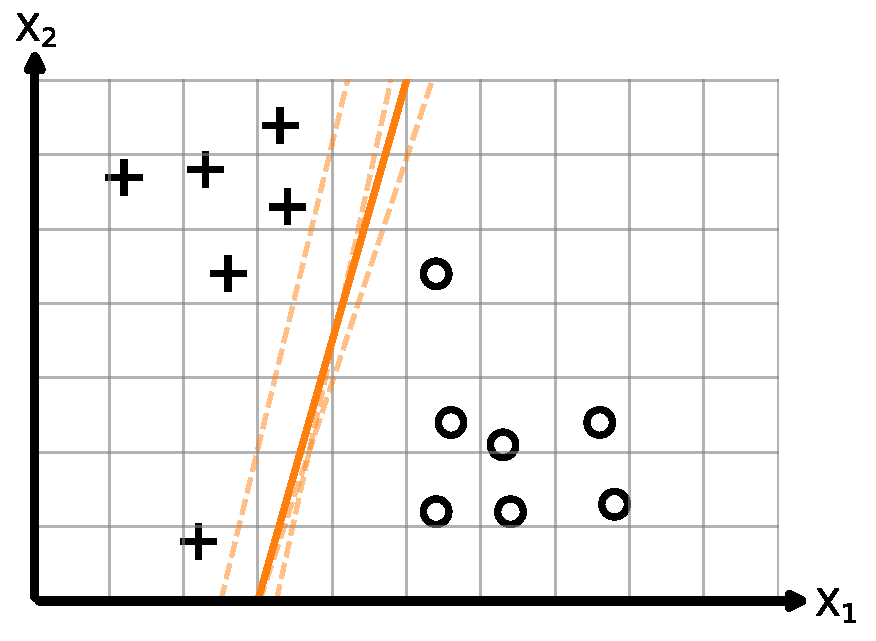
\includegraphics[width=0.7\textwidth]{code/result/problem6_1.pdf}
    \caption{Base Case}
    \label{fig:problem6_1}
\end{figure}

\textbf{Is the decision boundary unique?} No, the decision boundary is not unique. For linearly separable data,
there exists an infinite number of lines that can perfectly separate the two classes.
Any line within the margin between the two closest points of the opposite classes will achieve zero error on the training set.
In Figure \ref{fig:problem6_1}, all orange solid and dashed lines represent a feasible solution.

\textbf{How many classification errors?} The method makes \textbf{0} classification errors in this case, as the data is linearly separable.

\section[Regularize w0 heavily]{Regularize $w_0$ heavily}
When heavily regularize $w_0$ by minimizing $J_0(\mathbf{w}) = -\ell(\mathbf{w}, \mathcal{D}_{\text{train}}) + \lambda w_0^2$ with a very large $\lambda$,
the optimization forces $w_0 \approx 0$. The decision boundary equation $w_0 + w_1x_1 + w_2x_2 = 0$ simplifies to:
\[ w_1x_1 + w_2x_2 = 0 \]
This is the equation of a line that must pass through the origin $(0,0)$.
The model will find the best-fitting line through the origin to separate the classes, as shown below:

\begin{figure}[H]
    \centering
    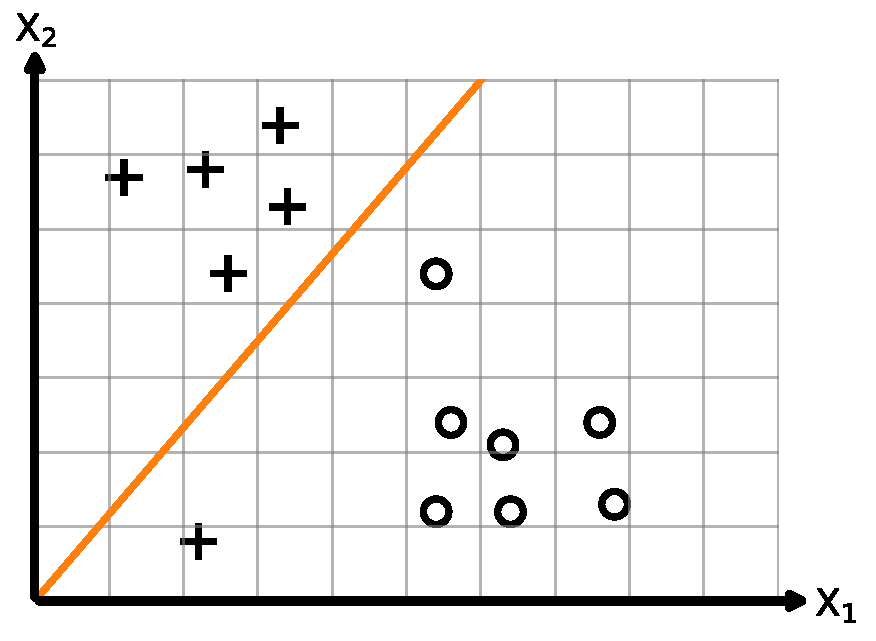
\includegraphics[width=0.7\textwidth]{code/result/problem6_2.pdf}
    \caption{Regularize $w_0$ heavily, with a decision boundary passing through the origin.}
    \label{fig:problem6_2}
\end{figure}

\textbf{How many classification errors?} In this case, it is possible to perfectly divide the classes
with a line passing through the origin, so the classification error will be $\textbf{0}$, as shown in the Figure \ref{fig:problem6_2}.

\section[Regularize w1 heavily]{Regularize $w_1$ heavily}
When we heavily regularize $w_1$, the optimization forces $w_1 \approx 0$. The decision boundary equation becomes:
\[ w_0 + w_2x_2 = 0 \quad \implies \quad x_2 = -\frac{w_0}{w_2} \]
This is the equation of a horizontal line. The model will find the best horizontal line that separates the two classes.

\begin{figure}[H]
    \centering
    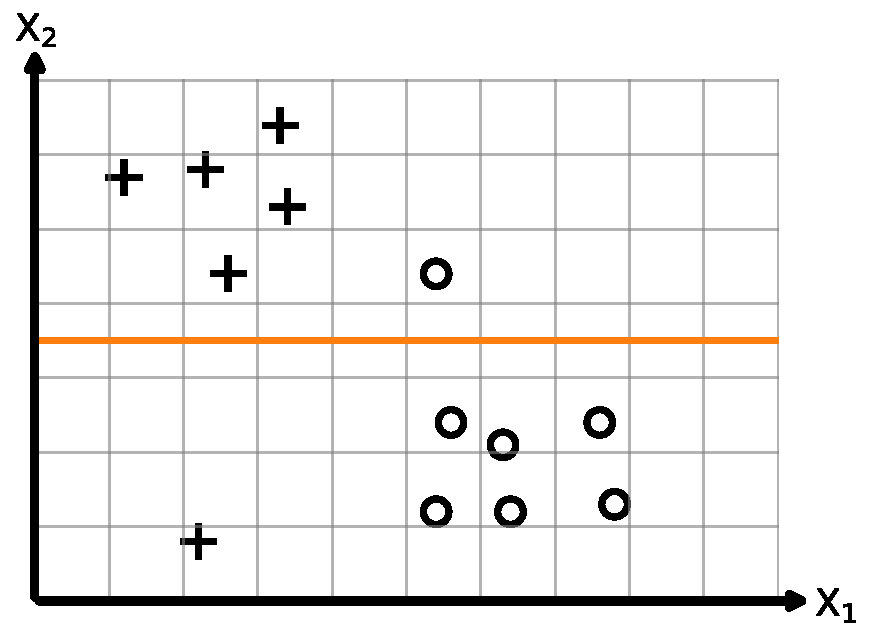
\includegraphics[width=0.7\textwidth]{code/result/problem6_3.pdf}
    \caption{Regularize $w_1$ heavily, with a decision boundary being a horizontal line.}
    \label{fig:problem6_3}
\end{figure}

\textbf{How many classification errors?} In this case, it's impossible to perfectly separate the classes with a horizontal line;
the optimal classification error will be $\textbf{2}$, as Figure \ref{fig:problem6_3}.

\section[Regularize w2 heavily]{Regularize $w_2$ heavily}
When we heavily regularize $w_2$, the optimization forces $w_2 \approx 0$. The decision boundary equation becomes:
\[ w_0 + w_1x_1 = 0 \quad \implies \quad x_1 = -\frac{w_0}{w_1} \]
This is the equation of a vertical line. The model will find the best vertical line that separates the two classes.

\begin{figure}[H]
    \centering
    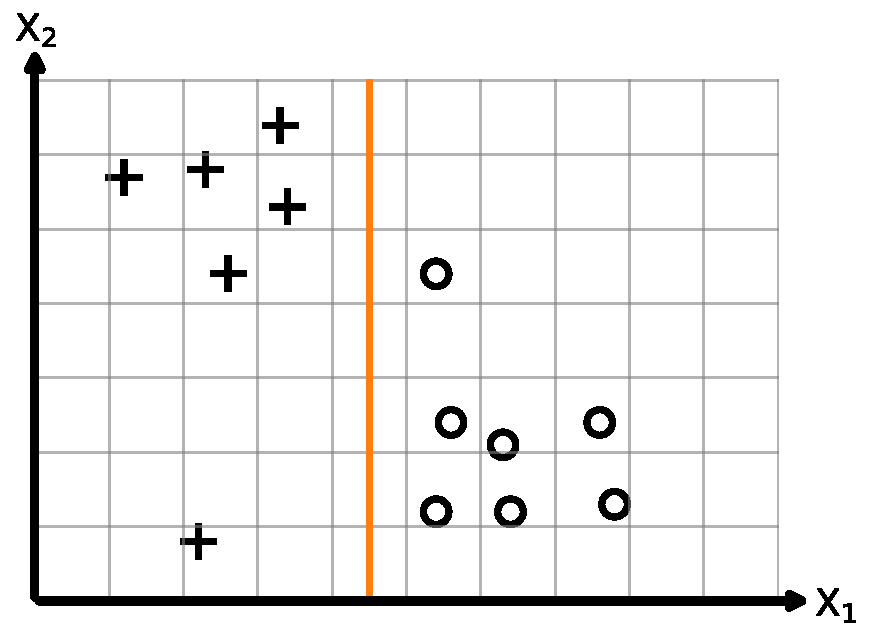
\includegraphics[width=0.7\textwidth]{code/result/problem6_4.pdf}
    \caption{Regularize $w_2$ heavily, with a decision boundary being a vertical line.}
    \label{fig:problem6_4}
\end{figure}

\textbf{How many classification errors?} In this case, it's possible to perfectly separate the classes with a vertical line,
so the optimal classification error will be $\textbf{0}$, as shown in the Figure \ref{fig:problem6_4}.

\chapter{Problem 7: Logistic Regression vs. LDA/QDA}
\section[GaussI vs. LinLog]{GaussI vs. LinLog: $L(\text{GaussI}) \le L(\text{LinLog})$}
The posterior probability for the GaussI model takes the form $p(y=1|x) = \sigma(\beta_0 + \beta^\top x)$.
This is because the log-odds, $\log \frac{p(x|y=1)p(y=1)}{p(x|y=0)p(y=0)}$, simplifies to a linear function of $x$
when the covariances are shared identity matrices. This function form is exactly the same as the LinLog model.

However, LinLog is trained by directly maximizing the conditional log-likelihood $L(M)$, while GaussI is trained by maximizing the joint log-likelihood.
Since the family of functions representable by LinLog contains the posterior distributions of GaussI,
and LinLog directly optimizes the metric in question,
it must achieve a conditional log-likelihood at least as high as GaussI.

\section[GaussX vs. QuadLog]{GaussX vs. QuadLog: $L(\text{GaussX}) \le L(\text{QuadLog})$}
The posterior probability for the GaussX model has log-odds that are a quadratic function of $x$,
because the $x^\top \Sigma_c^{-1} x$ terms do not cancel when $\Sigma_1 \neq \Sigma_0$.
This means the posterior is of the form $p(y=1|x) = \sigma(\beta_0 + \beta^\top x + x^\top A x)$,
which is exactly the functional form of the QuadLog model.

For the same reason as in the previous part,
since QuadLog directly maximizes the conditional log-likelihood over a model family that includes the posteriors of GaussX,
it will always achieve a value of $L(M)$ greater than or equal to that of GaussX.

\section[LinLog vs. QuadLog]{LinLog vs. QuadLog: $L(\text{LinLog}) \le L(\text{QuadLog})$}
The LinLog model is a special case of the QuadLog model where the quadratic coefficients are all zero.
This means the LinLog model family is nested within the QuadLog family.
When maximizing the same objective function ($L(M)$),
a more expressive model (QuadLog) can always achieve a likelihood at least as high as a less expressive, nested model (LinLog),
since it can simply learn to set the extra parameters to zero to replicate the simpler model's best solution.

\section[GaussI vs. QuadLog]{GaussI vs. QuadLog: $L(\text{GaussI}) \le L(\text{QuadLog})$}
$L(\text{GaussI}) \le L(\text{LinLog}) \le L(\text{QuadLog})$

\section[L(M) vs R(M)]{$L(M)$ vs. $R(M)$}
The conditional log-likelihood $L(M)$ measures the quality of the probabilistic predictions,
rewarding models that assign high probability to the correct class.

The misclassification rate $R(M)$ only depends on whether the predicted probability for the correct class is greater than 0.5 (for binary classification).

Model $M$ has the potential (and in fact, always does) to improve its overall probability estimates at the expense of misclassifying some data points,
thus leading to both $L(M)$ and $R(M)$ increasing simultaneously.

\chapter{Problem 8: MLE \& Model Optim: Grad Descent \& Newton's Method}
\section{Log-Likelihood Derivation}
The likelihood function $L(\beta)$ is the probability of observing the entire $N$ independent choices $\{y_i\}_{i=1}^N$.
Which is the product of the probabilities of each individual choice:
\[ L(\beta) = \prod_{i=1}^N p(y_i | x_i; \beta) \]
with the Multinomial Logit (MNL) model probability, we have:
\begin{align*}
    L(\beta)                     & = \prod_{i=1}^{N} \frac{\exp(\beta^\top x_{iy_i})}{\sum_{l \in C_i} \exp(\beta^\top x_{il})}                                   \\
    \ell(\beta) = \log(L(\beta)) & = \log \left( \prod_{i=1}^{N} \frac{\exp(\beta^\top x_{iy_i})}{\sum_{l \in C_i} \exp(\beta^\top x_{il})} \right)               \\
                                 & = \sum_{i=1}^{N} \left[ \log(\exp(\beta^\top x_{iy_i})) - \log \left( \sum_{l \in C_i} \exp(\beta^\top x_{il}) \right) \right] \\
                                 & = \sum_{i=1}^{N} \left[ \beta^\top x_{iy_i} - \log \left( \sum_{l \in C_i} \exp(\beta^\top x_{il}) \right) \right]
\end{align*}

\section{Gradient and Update Rules}
\subsection{Gradient}
To find the gradient $\nabla\ell(\beta)$, we need to differentiate $\ell(\beta)$ with respect to $\beta$:
\begin{align*}
    \nabla\ell(\beta) & = \nabla \sum_{i=1}^{N} \left[ \beta^\top x_{iy_i} - \log \left( \sum_{l \in C_i} \exp(\beta^\top x_{il}) \right) \right]         \\
                      & = \sum_{i=1}^{N} \left[ \nabla(\beta^\top x_{iy_i}) - \nabla \log \left( \sum_{l \in C_i} \exp(\beta^\top x_{il}) \right) \right]
\end{align*}
In which, the first term is straightforward $\nabla(\beta^\top x_{iy_i}) = x_{iy_i}$.
For the second term, let $S_i(\beta) = \sum_{l \in C_i} \exp(\beta^\top x_{il})$, we have:
\begin{align*}
    \nabla \log(S_i(\beta)) & = \frac{1}{S_i(\beta)} \nabla S_i(\beta)                                                                                                     \\
                            & = \frac{1}{\sum_{l \in C_i} \exp(\beta^\top x_{il})} \nabla \left( \sum_{l \in C_i} \exp(\beta^\top x_{il}) \right)                          \\
                            & = \frac{1}{\sum_{l \in C_i} \exp(\beta^\top x_{il})} \sum_{l \in C_i} \left( \exp(\beta^\top x_{il}) \cdot \nabla(\beta^\top x_{il}) \right) \\
                            & = \frac{1}{\sum_{l \in C_i} \exp(\beta^\top x_{il})} \sum_{l \in C_i} \exp(\beta^\top x_{il}) x_{il}                                         \\
                            & = \sum_{l \in C_i} \frac{\exp(\beta^\top x_{il})}{\sum_{k \in C_i} \exp(\beta^\top x_{ik})} x_{il}                                           \\
                            & = \sum_{l \in C_i} P(y_i = l | C_i, {x_{ik}}) x_{il}
\end{align*}
Which is the expectation of $x_{il}$ over the choices in set $C_i$, according to the model's predicted probabilities.
Thus, the overall gradient is:
\[ \nabla\ell(\beta) = \sum_{i=1}^{N} \left( x_{iy_i} - \sum_{l \in C_i} P(y_i = l | C_i) x_{il} \right) \]

\subsection{Update Rules}
\begin{itemize}
    \item \textbf{Gradient Descent (GD):} This is a gradient ascent algorithm since we are maximizing the log-likelihood. The update rule is:
          \[ \beta^{(t+1)} = \beta^{(t)} + \eta \nabla\ell(\beta^{(t)}) \]
          where $\eta > 0$ is the learning rate.
    \item \textbf{Newton's Method:} This method uses the Hessian matrix $H(\beta) = \nabla^2 \ell(\beta)$, which is the matrix of second partial derivatives. The update rule is:
          \[ \beta^{(t+1)} = \beta^{(t)} - [H(\beta^{(t)})]^{-1} \nabla\ell(\beta^{(t)}) \]
          The Hessian for the MNL log-likelihood is:
          \[ H(\beta) = -\sum_{i=1}^{N} \left( \sum_{l \in C_i} P_l x_{il} x_{il}^\top - \left(\sum_{l \in C_i} P_l x_{il}\right) \left(\sum_{l \in C_i} P_l x_{il}\right)^\top \right) \]
          where $P_l = P(y_i = l | C_i)$. The term inside the parenthesis is the covariance matrix of the feature vectors $x_{il}$
          under the model's probability distribution for user $i$.
          Since the log-likelihood function for the MNL model is concave,
          the Hessian $H(\beta)$ is negative semidefinite, ensuring that Newton's method moves towards a maximum.
\end{itemize}

\section{GD vs. Newton's Method}
\subsection{Adjustable Parameters}
As mentioned earlier, gradient descent (GD) has one key adjustable hyperparameter: the learning rate $\eta$.
Newton's method, in its pure form, does not have a learning rate\footnotemark,
The step size and direction are entirely determined by the gradient and the inverse Hessian matrix.
\footnotetext{In practice, a step size parameter (or damping parameter) is sometimes introduced to ensure stability, leading to the ``damped'' Newton's method.}

\subsection{Convergence Speed}
Newton's method typically converges much faster than gradient descent because it is a second-order method (using gradient and curvature (Hessian matrix) information),
which is equivalent to fitting the objective function with a quadratic function at each update and then directly ``jumping'' to the optimal value.

Gradient descent, on the other hand, is a first-order method (using only the gradient),
which is significantly slower.

However, the computational cost per step of Newton's method is much higher
because it requires computing and inverting a $d \times d$ Hessian matrix,
which requires $O(d^3)$ operations. Thus, in terms of wall-clock time, Newton's method may not necessarily converge faster.

\textit{Fun fact: A realistic example is the PPO and TRPO algorithms in reinforcement learning.
    The latter requires computing the Fisher information matrix (the Hessian matrix of KL divergence) each step,
    while the former is a simplified version that only needs a constrained gradient information (first-order).
    Experiments have shown that the former converges faster than the latter on various tasks.}

\chapter{Problem 9: Computing the Posterior Predictive}
Let's first review the core of Bayesian Posterior Predictive: first updating our beliefs about parameters $\theta$ after observing data $\mathcal{D}$.
This is governed by Bayes' theorem:
\[ p(\theta | \mathcal{D}) = \frac{p(\mathcal{D} | \theta) p(\theta)}{p(\mathcal{D})} \propto p(\mathcal{D} | \theta) p(\theta) \]
where $p(\theta)$ is the prior, $p(\mathcal{D} | \theta)$ is the likelihood, and $p(\theta | \mathcal{D})$ is the posterior.
For prediction on a new data point $x_*$, we compute the posterior predictive distribution by marginalizing over the posterior of the parameters:
\[ p(y_* | x_*, \mathcal{D}) = \int p(y_* | x_*, \theta) p(\theta | \mathcal{D}) d\theta \]


For our model $y = \boldsymbol{w}^\top \phi(x) + \epsilon$, we have:
\begin{itemize}
    \item \textbf{Prior}: A Gaussian prior on the weights $\boldsymbol{w}$:
          \[ p(\boldsymbol{w}) = \mathcal{N}(\boldsymbol{w} | \breve{\boldsymbol{w}}, \breve{\boldsymbol{\Sigma}}) = \mathcal{N}(\boldsymbol{w} | \boldsymbol{0}, \tau^2 \boldsymbol{I}) \]
          where $\breve{\boldsymbol{w}}$ is the prior mean and $\breve{\boldsymbol{\Sigma}}$ is the prior covariance matrix.

    \item \textbf{Likelihood}: A Gaussian likelihood for the observed data $\mathcal{D}$:
          \[ p(\mathcal{D} | \boldsymbol{w}, \sigma^2) = \prod_{n=1}^N p(y_n | x_n, \boldsymbol{w}, \sigma^2) = \prod_{n=1}^N \mathcal{N}(y_n | \boldsymbol{w}^\top \phi(x_n), \sigma^2) = \mathcal{N}(\boldsymbol{y} | \boldsymbol{w}^\top \phi(\boldsymbol{x}), \sigma^2 \boldsymbol{I}_N) \]
          where $\boldsymbol{I}_N$ is the $N \times N$ identity matrix. We can then use Bayes rule to derive the posterior:
          \begin{align*}
              p(\boldsymbol{w} | \mathcal{D}, \sigma^2) & \propto p(\mathcal{D} | \boldsymbol{w}, \sigma^2) p(\boldsymbol{w})                                                                                                                   \\
                                                        & = \mathcal{N}(\boldsymbol{y} | \boldsymbol{w}^\top \phi(\boldsymbol{x}), \sigma^2 \boldsymbol{I}_N) \mathcal{N}(\boldsymbol{w} | \breve{\boldsymbol{w}}, \breve{\boldsymbol{\Sigma}}) \\
                                                        & = \mathcal{N}(\boldsymbol{w} | \wideparen{\boldsymbol{w}}, \wideparen{\boldsymbol{\Sigma}})
          \end{align*}
          where
          \begin{align*}
              \wideparen{\boldsymbol{w}}      & = \wideparen{\boldsymbol{\Sigma}} (\breve{\boldsymbol{\Sigma}}^{-1} \breve{\boldsymbol{w}} + \frac{1}{\sigma^2} \phi(\boldsymbol{x})^\top \boldsymbol{y}) \\
              \wideparen{\boldsymbol{\Sigma}} & = (\breve{\boldsymbol{\Sigma}}^{-1} + \frac{1}{\sigma^2} \phi(\boldsymbol{x})^\top \phi(\boldsymbol{x}))^{-1}
          \end{align*}
          are the posterior mean and covariance matrix, respectively.
\end{itemize}

Thus, the posterior predictive distribution is:
\begin{align*}
    p(y_* | x_*, \mathcal{D}) & = \int p(y_* | x_*, \boldsymbol{w}, \sigma^2) p(\boldsymbol{w} | \mathcal{D}) d\boldsymbol{w}                                                                               \\
                              & = \int \mathcal{N}(y_* | \boldsymbol{w}^\top \phi(x_*), \sigma^2) \mathcal{N}(\boldsymbol{w} | \wideparen{\boldsymbol{w}}, \wideparen{\boldsymbol{\Sigma}}) d\boldsymbol{w} \\
                              & = \mathcal{N}(y_* | \wideparen{\boldsymbol{w}}^\top \phi(x_*), \wideparen{\sigma}^2)
\end{align*}
where $\wideparen{\sigma}^2 = \sigma^2 + \phi(x_*)^\top \wideparen{\boldsymbol{\Sigma}} \phi(x_*)$.

\newpage
\begin{figure}[H]
    \centering
    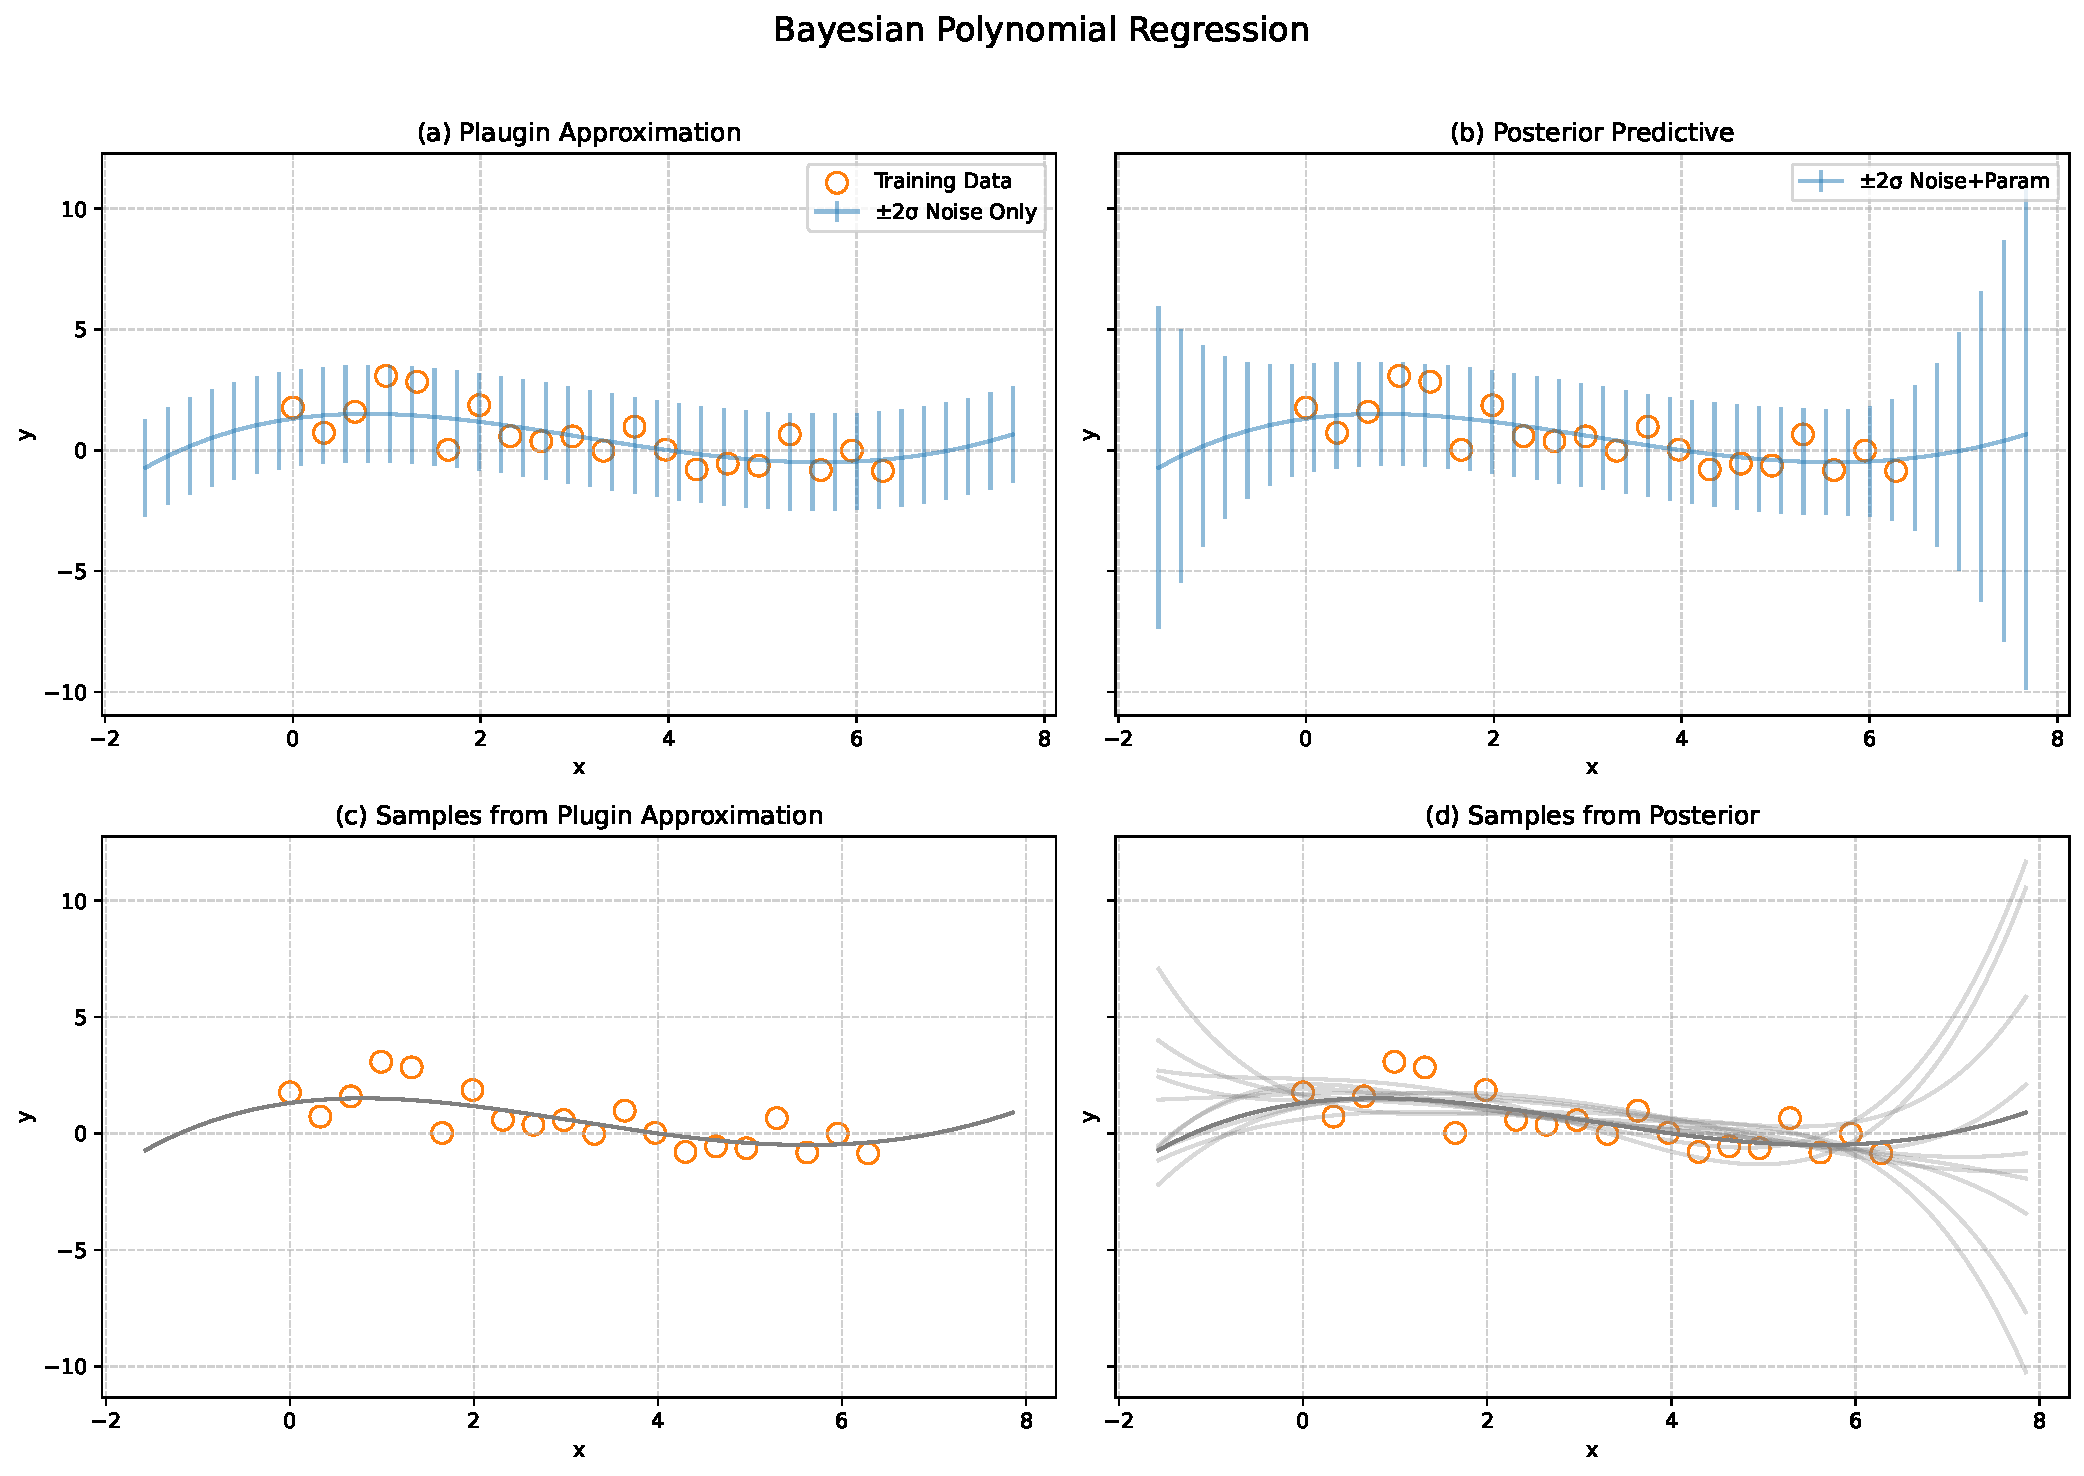
\includegraphics[width=\textwidth]{code/result/problem9.pdf}
    \caption{(a) Plugin approximation to predictive density (we plug in the MLE of the parameters) when fitting a second degree polynomial to some 1d data.
        (b) Posterior predictive density, obtained by integrating out the parameters. Black curve is posterior mean, error bars are 2 standard deviations of the posterior predictive density.
        (c) sample from the plugin approximation to posterior predictive distribution.
        (d) 10 samples from the true posterior predictive distribution. With heavy color is the plugin one.}
    \label{fig:problem9}
\end{figure}

\chapter{Programming I}
\section{Greedy}
\begin{align*}
    \mathcal{A}^{(6)} & = \{1, 2, 3, 4, 8, 10\} \\
    \beta^{(6)}       & = \begin{pmatrix}
                              5.10084     \\
                              13.2019937  \\
                              -9.09464524 \\
                              9.34579237  \\
                              12.18458507 \\
                              0.          \\
                              0.          \\
                              0.          \\
                              12.65362554 \\
                              0.          \\
                              -7.42805947
                          \end{pmatrix}
\end{align*}

\section{Ridge}
\begin{align*}
    \lambda^*                                    & = 0.0125             \\
    \beta^*                                      & = \begin{pmatrix}
                                                         5.10084     \\
                                                         13.15618925 \\
                                                         -9.32951139 \\
                                                         9.00778597  \\
                                                         12.38224078 \\
                                                         5.02341763  \\
                                                         -3.28072049 \\
                                                         -4.02556128 \\
                                                         12.82172388 \\
                                                         -4.93322552 \\
                                                         -7.34490684
                                                     \end{pmatrix}     \\
    \|y_{\text{true}} - y_{\text{pred}}\|_2^2    & = 35.8893064587282   \\
    \|\hat{\beta}^{\text{Ridge}} - \beta^*\|_2^2 & = 24.016307771599163
\end{align*}
% 标记最后一页用于总页数计算
\label{LastPage}
\end{document}

